\documentclass{scrartcl}

\usepackage[utf8]{inputenc} % Unicode support (Umlauts etc.)
\usepackage{hyperref} % Add a link to your document
\usepackage{graphicx} % Add pictures to your document
\usepackage{listings} % Source code formatting and highlighting
\usepackage[top=75px, bottom=75px, left=85px, right=85px]{geometry} % Change page borders
\usepackage{graphicx}

\begin{document}

\title{Computational Intelligence:
\\Report assignment 1}
\date{\today{}}

\author{
    \begin{tabular}{l r}
    	\\Tjitte de Jong
	\\Boris Mulder
        \\Max Spanoghe - 4331834
            \end{tabular}
  }
  
  \maketitle \thispagestyle{empty} \pagebreak
  
  \section{Questions}
  Here we will answer the questions of the first assigment.
  
  \subsection{}
  Our group will be using 10 input neurons because the objects have ten different features.
  
  \subsection{}
  The script should have 7 output neurons because there are 7 different categories for the objects.
  Hence, this is the amount of possible outcomes.
  
  \subsection{}
  We will create a hidden layer with 12 hidden neurons. This is still a guess,  but we can try to change
  this amount later.
  
  \subsection{}
  We will use the sigmoid function because we we think this will give the best result. We can calculate the
  errors in the end much more precisely if we use this function.
  
  \subsection{}
  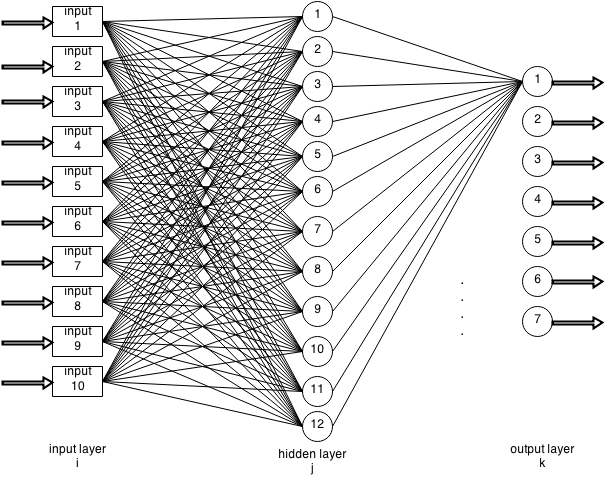
\includegraphics[scale = 0.7]{network.png}
  
  \subsection{}
  It is important that the program has a set of data as input at the targets for validation because we are dealing with a supervised neural network. This means we have inputs and also outputs to actually train the network. The test set is used after the program trained itself to check weather the weights also work for unused data in the training. If it is trained well, the program should be able to recognize the categories of the objects in the test set.
  
  \subsection{}
  You can tests the program's performance by using such a test set. To make sure you don't find a local minimum or have smaller or higher errors, you should actually do cross validation (maybe k-fold). Here you divide your data in smaller sets and change their role(training set, ...). Then you should take the avg error and this is a better way to actually know the performance.
  
  \subsection{}
  Our group thinks there are different ways to do this. One way is to set a threshold on the error. For example, if the error is lower than x, the weights are set correctly. In other words, you can give criteria on when the weights are good enough.
  
  \subsection{}
  With different initial weights our program gets different results. This happens because with the different initial weights, the weights can find another way to a maybe lower error. For example, some weights can be trained but get a local minimum as error, while other trained weights have a lower error. It depends on where you started.
  
  
\end{document}